% Drawing 154/06-11 -- folder 154, batch 06, archive page 114 (PDF page 115).
% Transcription: page de dessins : en haut à gauche, un hexagone et un pentagone vert clair accolés, des croix rouges sur les arêtes ; au crayon, deux cercles tangents traversés de courbes, le point de contact marqué, avec les accolades $\alpha_0$, $\alpha_1$, $\alpha_2$, $\alpha''$ et « $n - \nu$ » ; en haut à droite, un croquis au crayon d'un pentagone et d'une droite coupée de droites, avec un arc vert clair au-dessous. En bas, un huit au crayon marqué « $N' = N - 1$ », des arcs vert clair aux points marqués « $1$ », « $2$ », « $3$ » (avec des signes $\sim$), des cercles au crayon, et à droite un huit en couleur (vert clair, vert foncé, arcs renforcés en brun) aux arcs marqués « $1$ », « $1{+}$ », « $3$ », « $13$ »
% Kind: hexagon and pentagon with red crosses; pencil tangent circles with braces; arcs with numbered points; a figure eight. Method 2 (schematic redraw from the facsimile). Status: partial.
% Notes: Page of drawings, read from the page view. Top left, a light green hexagon and pentagon glued along an edge, red crosses on the edges. In pencil, two tangent circles crossed by curves, the point of contact marked, with the braces alpha_0, alpha_1, alpha_2, alpha'' and « n - nu » (given as labels). Top right, a pencil sketch of a pentagon and of a line cut by lines, with a light green arc below. Bottom: a pencil figure eight marked « N' = N - 1 », light green arcs with points marked 1, 2, 3 (with ~ signs; placed approximately), pencil circles, and on the right a figure eight in colour (light green, dark green, arcs reinforced in brown) with arcs marked 1, 1+, 3, 13 (placed approximately). Still differs from the facsimile: Bottom: a pencil figure eight marked « N' = N - 1 », light green arcs with points marked 1, 2, 3 (with ~ signs; placed approximately), pencil circles, and on the right a figure eight in colour (light green, dark green, arcs reinforced in brown) with arcs marked 1, 1+, 3, 13 (placed approximately).
% Coordinates: 1 unit = 1 mm = 1/100 of the crop width (bbox in page fractions: [0.148, 0.111, 0.937, 0.502]).
% Redrawn by Claude (claude-opus-5-5), issue #73, 2026-11-07; not checked by a human; not compiled (no TeX in the session).
% Revised by Claude (claude-opus-5-5) 2026-11-09 (issue #128) after Michel's check: vertices snapped to exact intersections (drawn points on their lines, meeting ends on the stroke they meet, near-concurrent lines through one computed point, curve ends on their rim); labels at \small as in folder 80 batch 3. Status: partial.
% Rights: reproduces part of the work -- behind RENDER_TRANSCRIPTS, never published by itself.
\documentclass[tikz,border=3pt]{standalone}
\usepackage{amsmath,amssymb}
\usetikzlibrary{patterns,arrows.meta}
\tikzset{Or/.style={orange!90!black}, Ye/.style={yellow!80!orange}, Lg/.style={green!60!black!70}, Dg/.style={green!45!black}, Br/.style={brown!80!black}, Rd/.style={red!85!black}, Bl/.style={blue!70!black}, Gy/.style={black!40}, pencil/.style={black!45}, struck/.style={black!35}, mark/.style={circle,draw,inner sep=1.3pt}, pt/.style={circle,fill,inner sep=0.9pt}, opt/.style={circle,draw,fill=white,inner sep=1.1pt}}
\begin{document}
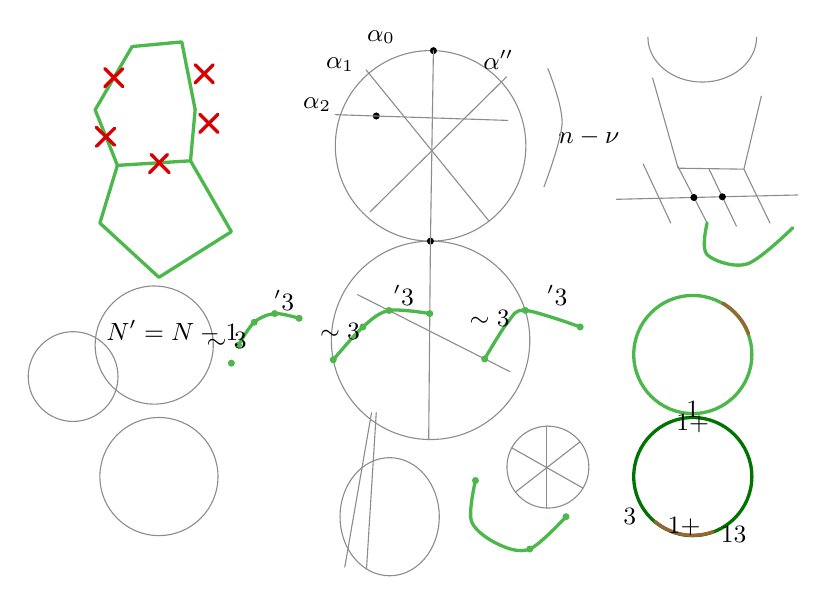
\begin{tikzpicture}[x=1mm,y=1mm,line cap=round,line join=round,font=\scriptsize]
\draw[Lg,very thick] (14.39,-2.89) -- (20.7,-2.3) -- (22.4,-10.9) -- (21.81,-17.4) -- (12.53,-17.98) -- (9.7,-10.93) -- cycle;
\draw[Lg,very thick] (12.53,-17.98) -- (10.3,-25.3) -- (17.8,-32.2) -- (27,-26.4) -- (21.81,-17.4);
\draw[Rd,very thick] (10.92,-5.68) -- (13.22,-7.98);
\draw[Rd,very thick] (10.91,-8.01) -- (13.21,-5.71);
\draw[Rd,very thick] (22.4,-5.2) -- (24.7,-7.5);
\draw[Rd,very thick] (22.4,-7.5) -- (24.7,-5.2);
\draw[Rd,very thick] (9.85,-13.15) -- (12.17,-15.43);
\draw[Rd,very thick] (9.86,-15.56) -- (12.17,-13.27);
\draw[Rd,very thick] (23,-11.5) -- (25.3,-13.8);
\draw[Rd,very thick] (23,-13.8) -- (25.3,-11.5);
\draw[Rd,very thick] (16.81,-16.59) -- (19.09,-18.91);
\draw[Rd,very thick] (16.61,-18.91) -- (18.89,-16.59);
\draw[pencil] (52.3,-15.5) circle[radius=12.1];
\draw[pencil] (52.3,-40.2) circle[radius=12.6];
\node[pt] at (52.28,-27.6) {};
\node[pt] at (52.66,-3.41) {};
\node[pt] at (45.4,-11.71) {};
\draw[pencil] (40.2,-11.54) -- (62.1,-12.27);
\draw[pencil] (44.11,-5.85) -- (59.72,-25.05);
\draw[pencil] (44.6,-23.9) -- (61.94,-6.74);
\draw[pencil] (52.66,-3.41) -- (52.28,-27.6);
\draw[pencil] (52.28,-27.6) -- (52.06,-52.8);
\draw[pencil] (43.03,-34.4) -- (62.38,-44.18);
\node[inner sep=1pt] at (46,-1.7) {\small $\alpha_0$};
\node[inner sep=1pt] at (40.8,-5.2) {\small $\alpha_1$};
\node[inner sep=1pt] at (37.9,-10.3) {\small $\alpha_2$};
\node[inner sep=1pt] at (60.9,-4.6) {\small $\alpha''$};
\node[inner sep=1pt] at (72.4,-14.4) {\small $n-\nu$};
\draw[pencil] plot[smooth, tension=0.55] coordinates {(67.2,-5.7) (69,-12.6) (66.7,-20.7)};
\draw[pencil] (79.9,-1.7) arc[start angle=180, end angle=360, x radius=6.9, y radius=5.7];
\draw[pencil] (80.5,-6.9) -- (83.74,-18.34) -- (92.09,-18.46) -- (94.3,-9.2);
\draw[pencil] (75.9,-22.29) -- (98.9,-21.74);
\draw[pencil] (79.3,-17.8) -- (82.8,-25.3);
\draw[pencil] (83.64,-17.99) -- (87.42,-25.3);
\draw[pencil] (87.64,-18.4) -- (91.14,-25.7);
\draw[pencil] (92.09,-18.46) -- (95.4,-25.3);
\draw[Lg,very thick] plot[smooth, tension=0.55] coordinates {(87.42,-25.3) (87.4,-29.3) (92.5,-30.5) (98.3,-25.9)};
\node[pt] at (85.74,-22.06) {};
\node[pt] at (89.36,-21.97) {};
\draw[pencil] (6.9,-44.8) circle[radius=5.7];
\draw[pencil] (17.2,-40.8) circle[radius=7.5];
\draw[pencil] (17.8,-57.5) circle[radius=7.5];
\node[inner sep=1pt] at (19.5,-39.1) {\small $N'=N-1$};
\draw[Lg,very thick] plot[smooth, tension=0.55] coordinates {(27.9,-40.8) (29.9,-37.9) (32.5,-36.8) (35.6,-37.4)};
\node[pt,Lg] at (27,-43.1) {};
\node[pt,Lg] at (27.9,-40.8) {};
\node[pt,Lg] at (29.9,-37.9) {};
\node[pt,Lg] at (32.5,-36.8) {};
\node[pt,Lg] at (35.6,-37.4) {};
\node[inner sep=1pt] at (26.4,-40.2) {\small $\sim3$};
\node[inner sep=1pt] at (33.7,-35.1) {\small $'3$};
\draw[Lg,very thick] plot[smooth, tension=0.55] coordinates {(39.94,-42.67) (43.7,-38.5) (47.01,-36.41) (52.2,-36.8)};
\node[pt,Lg] at (39.94,-42.67) {};
\node[pt,Lg] at (43.7,-38.5) {};
\node[pt,Lg] at (47.01,-36.41) {};
\node[pt,Lg] at (52.2,-36.8) {};
\node[inner sep=1pt] at (40.8,-39.1) {\small $\sim3$};
\node[inner sep=1pt] at (48.9,-34.5) {\small $'3$};
\draw[Lg,very thick] plot[smooth, tension=0.55] coordinates {(59.17,-42.56) (62.1,-37.9) (64.31,-36.39) (71.3,-38.5)};
\node[pt,Lg] at (59.17,-42.56) {};
\node[pt,Lg] at (64.31,-36.39) {};
\node[pt,Lg] at (71.3,-38.5) {};
\node[inner sep=1pt] at (59.8,-37.4) {\small $\sim3$};
\node[inner sep=1pt] at (68.4,-34.5) {\small $'3$};
\draw[pencil] (47.1,-62.6) ellipse[x radius=6.3, y radius=7.5];
\draw[pencil] (44.8,-49.4) -- (41.4,-69);
\draw[pencil] (45.4,-49.4) -- (44.16,-69.23);
\draw[pencil] (67.2,-56.3) circle[radius=5.2];
\draw[pencil] (62.61,-53.85) -- (71.66,-58.97);
\draw[pencil] (63.08,-59.47) -- (71.28,-53.08);
\draw[pencil] (67.06,-51.1) -- (67.06,-61.5);
\draw[Lg,very thick] plot[smooth, tension=0.55] coordinates {(58,-58) (57.5,-63.2) (60.9,-66.1) (64.9,-66.7) (69.5,-62.6)};
\node[pt,Lg] at (58,-58) {};
\node[pt,Lg] at (69.5,-62.6) {};
\node[pt,Lg] at (64.9,-66.7) {};
\draw[Lg,very thick] (85.6,-42) ellipse[x radius=7.5, y radius=7.5];
\draw[Dg,very thick] (85.6,-57.5) ellipse[x radius=7.5, y radius=7.5];
\draw[Br,very thick] (92.7,-39.4) arc[start angle=20, end angle=60, x radius=7.5, y radius=7.5];
\draw[Br,very thick] (80.8,-63.2) arc[start angle=230, end angle=290, x radius=7.5, y radius=7.5];
\node[inner sep=1pt] at (85.6,-49) {\small $1$};
\node[inner sep=1pt] at (85.6,-50.8) {\small $1+$};
\node[inner sep=1pt] at (77.6,-62.6) {\small $3$};
\node[inner sep=1pt] at (84.5,-63.8) {\small $1+$};
\node[inner sep=1pt] at (90.8,-64.9) {\small $13$};
\end{tikzpicture}
\end{document}
